\documentclass[10pt,a4paper]{article}
\usepackage[utf8]{inputenc}
\usepackage[francais]{babel}
\usepackage[T1]{fontenc}
\usepackage{amsmath}
\usepackage{amsfonts}
\usepackage{amssymb}
\usepackage{graphicx}
\usepackage{enumitem}
\usepackage{lmodern}
\usepackage{listings}
\usepackage{color}
\usepackage{tikz}

\definecolor{mygreen}{rgb}{0,0.6,0}
\definecolor{mygray}{rgb}{0.5,0.5,0.5}
\definecolor{mymauve}{rgb}{0.58,0,0.82}

\lstset{ %
  backgroundcolor=\color{white},   % choose the background color; you must add \usepackage{color} or \usepackage{xcolor}
  basicstyle=\footnotesize,        % the size of the fonts that are used for the code
  breakatwhitespace=false,         % sets if automatic breaks should only happen at whitespace
  breaklines=true,                 % sets automatic line breaking
  captionpos=b,                    % sets the caption-position to bottom
  commentstyle=\color{mygreen},    % comment style
  deletekeywords={...},            % if you want to delete keywords from the given language
  escapeinside={\%*}{*)},          % if you want to add LaTeX within your code
  extendedchars=true,              % lets you use non-ASCII characters; for 8-bits encodings only, does not work with UTF-8
  frame=single,                    % adds a frame around the code
  keepspaces=true,                 % keeps spaces in text, useful for keeping indentation of code (possibly needs columns=flexible)
  keywordstyle=\color{blue},       % keyword style
  language=Java,                   % the language of the code
  morekeywords={*,...},            % if you want to add more keywords to the set
  numbers=left,                    % where to put the line-numbers; possible values are (none, left, right)
  numbersep=5pt,                   % how far the line-numbers are from the code
  numberstyle=\tiny\color{mygray}, % the style that is used for the line-numbers
  rulecolor=\color{black},         % if not set, the frame-color may be changed on line-breaks within not-black text (e.g. comments (green here))
  showspaces=false,                % show spaces everywhere adding particular underscores; it overrides 'showstringspaces'
  showstringspaces=false,          % underline spaces within strings only
  showtabs=false,                  % show tabs within strings adding particular underscores
  stepnumber=2,                    % the step between two line-numbers. If it's 1, each line will be numbered
  stringstyle=\color{mymauve},     % string literal style
  tabsize=4,                       % sets default tabsize to 2 spaces
  title=\lstname                   % show the filename of files included with \lstinputlisting; also try caption instead of title
}
\usepackage[left=2cm,right=2cm,top=2cm,bottom=2cm]{geometry}


\date{Jeudi 30 octobre 2014}
\author{Groupe 2.2}
\title{Mission 3 : Rapport Final}
\begin{document}
\maketitle
\section*{Introduction}
Dans cette mission, notre but était d'implémenter une application permettant d'accéder aux informations asociées à une revue scientifique dont on fournit un nom. Pour ce faire, il nous était demandé d'implémenter une solution utilisant une Map (non ordornné).

\section*{Description de l'implémentation}
Chaque publication scientifique est représentée par un objet Publication dont le constructeur reçoît une ligne correspondant à toutes les informations de la dite publication. Comme son nom l'indique, LightPublication représente une publication "plus légère" qui va nous permettre d'un stocker beaucoup en prennant moins de place que si on avait utilisé des Publication. Nous avons également une classe PublicationMap permet de créée une map de Publication, elle contient un constructeur qui crée deux HashMap, la première ayant comme clé le nom d'une publication et comme valeur des objet LightPublication, la deuxième ayant comme clé un entier et comme valeur le nom de la référence correspondant à sa clé. La classe PublicationMap permet d'ajouter une publication soit à partir d'une ligne du fichier de base, soit à partir d'un objet Publication. On ne peux récupérer une publication dans le Map à partir de son nom uniquement.

\subsection*{Diagramme de classe}
\begin{figure}[!h]
    \begin{center}
    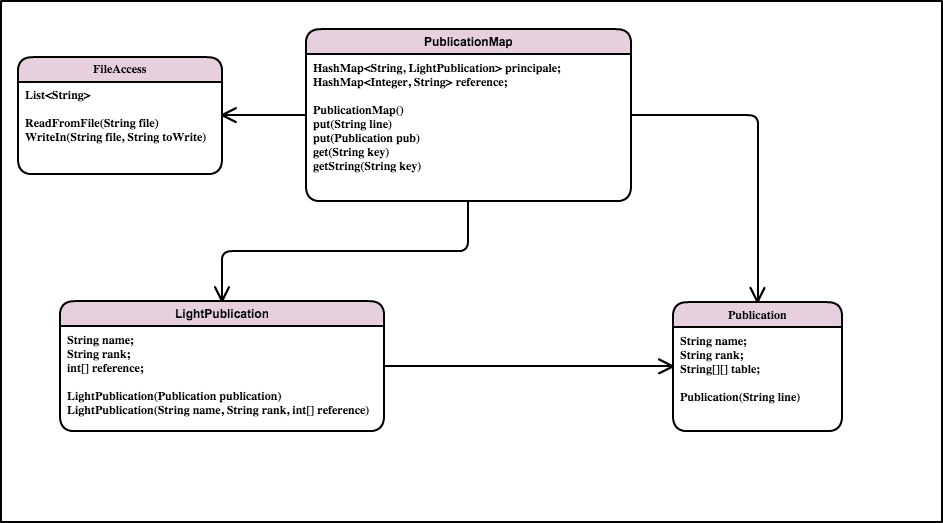
\includegraphics[scale=0.5]{Diagram.png}
    \caption{Diagramme de classe de notre programme.}
    \label{fig:ClassDiagram}
    \end{center}
\end{figure}
\newpage

\section*{Conclusion}
La décomposition des classes dans notre programme, aurait du faciliter la répartition des taches, l'utilisation de multiple classe permet de pouvoir être plus modulable. Tant au niveau de la repartition du travail, qu'au niveau de l'ajout de nouvelles fonctions pour adapter notre programme.
\end{document}